\subsection{Analisis Kondisi DecMed}

Analisis kondisi sistem dilakukan untuk mengidentifikasi komponen-komponen yang relevan dalam proses pemodelan ancaman. Analisis ini menggunakan Data Flow Diagram (DFD) yang menggambarkan entitas eksternal, proses, penyimpanan data, serta aliran data dalam sistem DecMed. Berdasarkan DFD tersebut akan dilakukan identifikasi aset, entry points, dan trust boundaries sebagai dasar analisis ancaman menggunakan metode STRIDE.

\begin{figure}[ht]
	\centering
	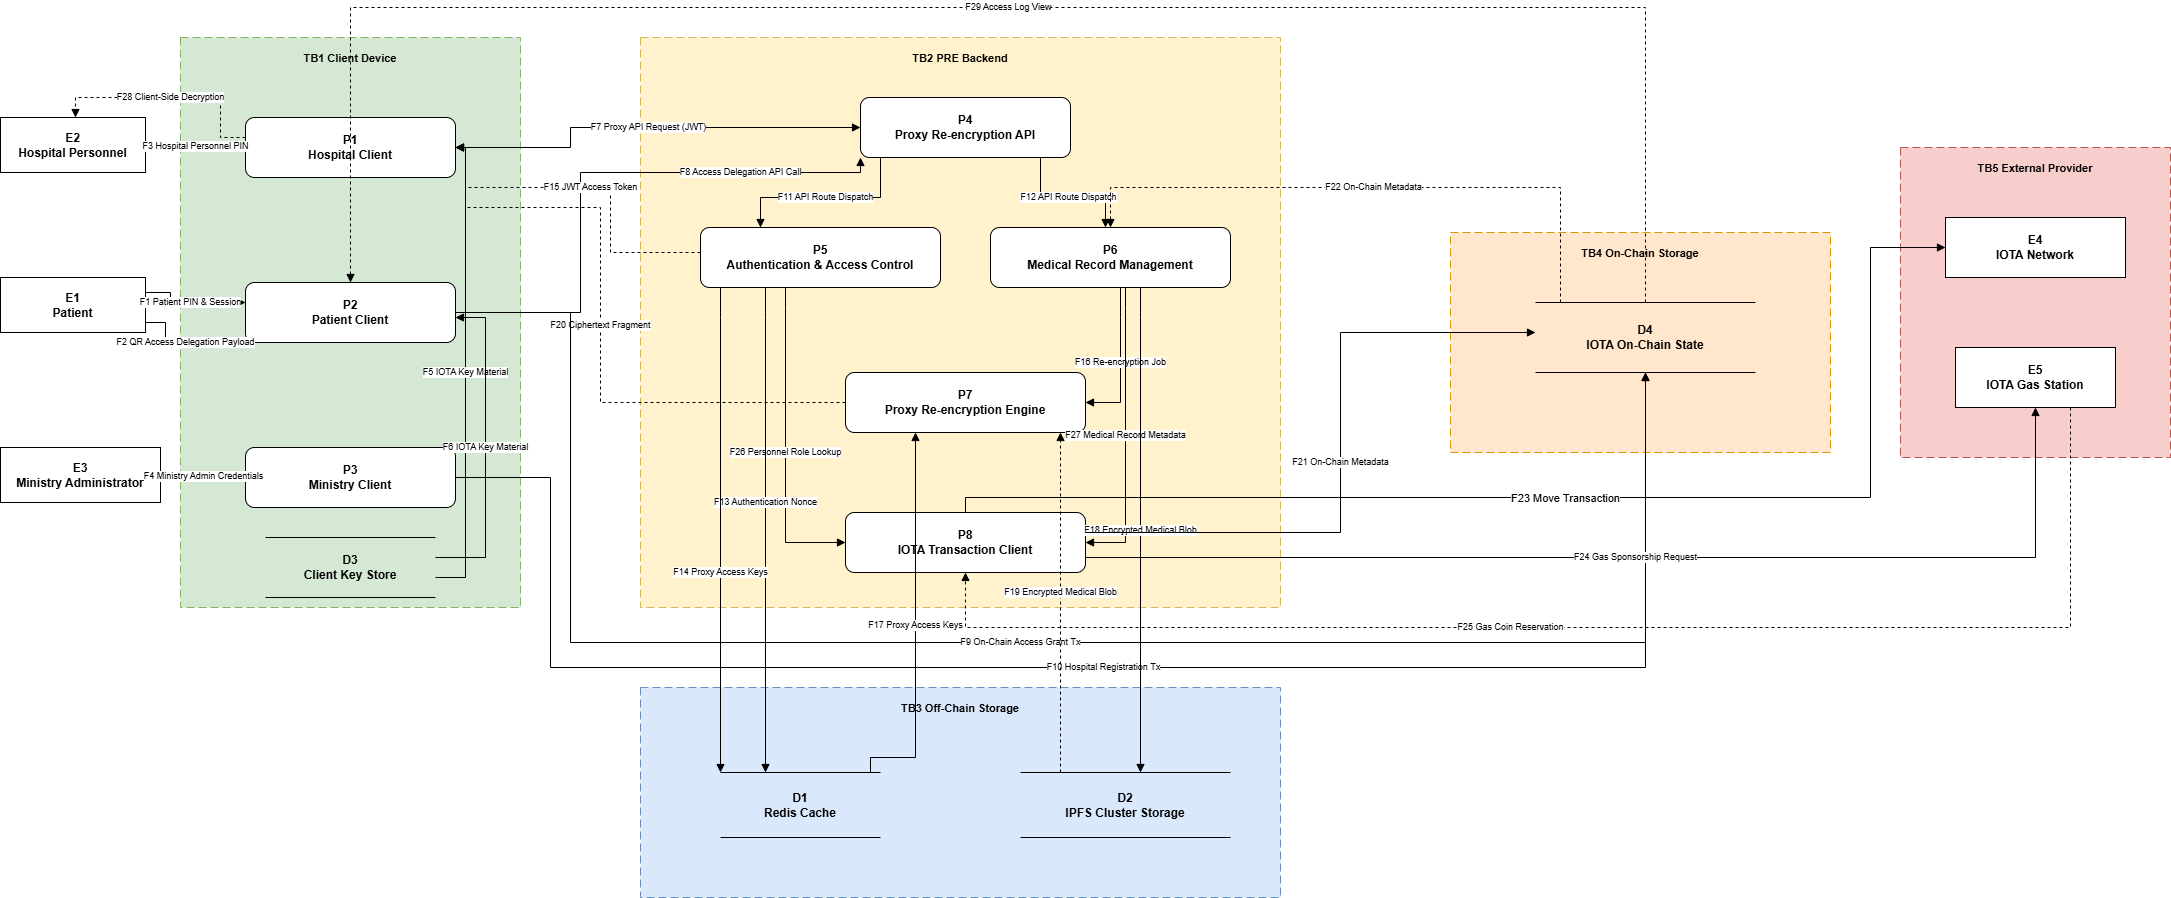
\includegraphics[width=1\textwidth]{resources/chapter-3/dfd-decmed.png}
	\caption{Data Flow Diagram (DFD) Sistem DecMed}
    \label{fig:dfd-decmed}
\end{figure}

Berdasarkan DFD pada Gambar~\ref{fig:dfd-decmed}, sistem DecMed terdiri atas beberapa komponen utama yang berinteraksi untuk mengelola data rekam medis pasien. Diagram tersebut memperlihatkan bagaimana data berpindah antar komponen serta lokasi penyimpanan data, sehingga dapat digunakan sebagai dasar untuk mengidentifikasi aset yang perlu dilindungi dan area yang berpotensi menjadi sumber ancaman.

\subsubsection{Identifikasi Aset}
Setelah struktur sistem dan aliran data dipetakan melalui DFD, langkah selanjutnya adalah mengidentifikasi aset yang memiliki nilai dan memerlukan perlindungan keamanan. Aset-aset tersebut mencakup data yang diproses oleh sistem maupun komponen infrastruktur yang mendukung operasional DecMed.

Aset data mencakup seluruh informasi, kredensial, kunci kriptografi, dan metadata yang diproses, disimpan, atau digunakan oleh sistem DecMed. Aset-aset ini memiliki tingkat sensitivitas yang tinggi karena berkaitan langsung dengan identitas pengguna, rekam medis pasien, serta mekanisme keamanan sistem. Daftar aset data yang teridentifikasi ditunjukkan pada Tabel~\ref{tab:aset-data}.

\begin{table}[htbp]
    \centering
    \caption{Daftar Aset Data dalam DecMed}
    \vspace{0.25cm}
    \label{tab:aset-data}
    \begin{tabular}{|p{2.5cm}|p{3.5cm}|p{8cm}|}
        \hline
        \textbf{Kode DFD} & \textbf{Nama Aset} & \textbf{Deskripsi} \\
        \hline
        D2, F18, F19 & Data Klinis (EMR) & Berisi data rekam medis pasien yang dienkripsi (Encrypted Medical Blob) dan disimpan di luar jaringan (off-chain) pada IPFS Cluster Storage. \\
        \hline
        D4, F10 & Data Administratif & Data registrasi rumah sakit (Hospital Registration Tx) dan identitas yang dicatat langsung pada IOTA On-Chain State. \\
        \hline
        D3, F1, F3 & Kredensial Personal \& PIN & Kredensial lokal (Patient PIN, Hospital Personnel PIN) yang diamankan pada Client Key Store untuk mengelola sesi pengguna. \\
        \hline
        D1, F5, F6, F14, F17 & Kunci Kriptografi \& PRE & IOTA Key Material dan Proxy Access Keys yang disimpan dalam Redis Cache (D1) dan Client Key Store (D3) untuk proses re-enkripsi. \\
        \hline
        F4 & Kredensial Admin & Kredensial rahasia yang dikirimkan oleh Ministry Administrator (E3) ke Ministry Client (P3) untuk konfigurasi awal sistem. \\
        \hline
        F7, F15 & Token Akses (JWT) & Bukti hak akses berbatas waktu (JWT Access Token) bagi klien untuk memanggil Proxy API Request. \\
        \hline
        D4, F9, F21, F22 & Metadata \& On-Chain Access Grant & Entri kapabilitas dan metadata on-chain yang disimpan di D4 (IOTA On-Chain State) yang krusial untuk audit log. \\
        \hline
        D1, F13 & Nonce & Nilai acak berumur pendek untuk otentikasi (Authentication Nonce) yang disimpan di Redis Cache guna mencegah replay attacks. \\
        \hline
    \end{tabular}
\end{table}

Selain aset data, DecMed juga bergantung pada berbagai komponen infrastruktur yang menjalankan fungsi operasional, keamanan, dan penyimpanan. Komponen-komponen ini berperan dalam pemrosesan transaksi, pengelolaan hak akses, penyimpanan data, serta komunikasi antarbagian sistem. Daftar aset infrastruktur yang menjadi objek analisis ditunjukkan pada Tabel~\ref{tab:aset-infrastruktur}.

\begin{table}[htbp]
    \centering
    \caption{Daftar Aset Infrastruktur dalam DecMed}
    \vspace{0.25cm}
    \label{tab:aset-infrastruktur}
    \begin{tabular}{|p{2.5cm}|p{3.5cm}|p{8cm}|}
        \hline
        \textbf{Kode DFD} & \textbf{Nama Aset} & \textbf{Deskripsi} \\
        \hline
        P1, P2, P3 & Aplikasi Klien & Antarmuka utama (Hospital, Patient, dan Ministry Client) yang memproses input pengguna dan operasi kriptografi lokal di dalam TB1. \\
        \hline
        P4, P5, P6, P7, P8 & PRE Backend & Middleware keamanan (TB2) yang mengeksekusi Proxy Re-Encryption (P7), Authentication (P5), dan berinteraksi dengan IOTA (P8). \\
        \hline
        E5 & Server Gas Station & Entitas penyedia eksternal yang bertugas mensponsori biaya transaksi (Gas Sponsorship Request) di jaringan IOTA. \\
        \hline
        D4 & IOTA On-Chain State & Layer 1 IOTA yang berfungsi sebagai Access Registry. Aset ini memvalidasi izin dan mencatat audit trail (log akses). \\
        \hline
        D1, D2 & Penyimpanan Off-Chain & Klaster IPFS Storage (D2) untuk menampung file EMR terenkripsi, serta Redis Cache (D1) untuk menampung data operasional berumur pendek. \\
        \hline
    \end{tabular}
\end{table}


\subsubsection{Identifikasi Entry Points}
Selain mengidentifikasi aset, penting untuk menentukan titik masuk (entry points) yang dapat digunakan oleh pengguna maupun pihak lain untuk berinteraksi dengan sistem. Titik masuk ini berpotensi menjadi jalur eksploitasi apabila tidak dilindungi dengan mekanisme keamanan yang memadai. Daftar entry points yang teridentifikasi dalam sistem DecMed ditunjukkan pada Tabel~\ref{tab:entry-points}.

\begin{table}[htbp]
    \centering
    \caption{Daftar Titik Masuk (Entry Points) dalam DecMed}
    \vspace{0.25cm}
    \label{tab:entry-points}
    \begin{tabular}{|p{2.5cm}|p{3.5cm}|p{8cm}|}
        \hline
        \textbf{Kode DFD} & \textbf{Nama Entry Point} & \textbf{Deskripsi} \\
        \hline
        P2 & Aplikasi Patient Client & Titik interaksi pasien (E1) untuk mendelegasikan akses dan memasukkan PIN ke dalam sistem klien lokal. \\
        \hline
        F2 & Payload QR Code & Titik pertukaran data awal (QR Access Delegation Payload) untuk transfer hak akses dari pasien ke faskes. \\
        \hline
        P1 & Aplikasi Hospital Client & Titik masuk bagi Hospital Personnel (E2) untuk mengakses dan menginput EMR melalui antarmuka desktop/lokal. \\
        \hline
        P3 & Aplikasi Ministry Client & Titik masuk administratif tempat Ministry Administrator (E3) memasukkan kredensial dan meregistrasi faskes. \\
        \hline
        P4 & Proxy Re-encryption API & Titik masuk utama pada PRE Backend (TB2) yang menerima request (F7) dan pendelegasian akses (F28) dari layer klien. \\
        \hline
        E5 & IOTA Gas Station API & Titik komunikasi yang menerima Gas Sponsorship Request (F24) dari PRE Backend (P8) ke penyedia eksternal. \\
        \hline
        E4, D4 & IOTA Network & Titik masuk jaringan buku besar terdistribusi untuk menerima eksekusi Move Transaction (F23) dari IOTA Transaction Client. \\
        \hline
        D2 & Antarmuka IPFS & Gateway penyimpanan tempat blob medis terenkripsi (F18) diunggah dan diunduh (F19). \\
        \hline
        D1 & Redis Cache & Antarmuka basis data internal yang menerima aliran masuk Authentication Nonce (F13) dari Authentication \& Access Control (P5). \\
        \hline
    \end{tabular}
\end{table}

\subsubsection{Identifikasi Trust Boundaries}
Dalam DFD, beberapa aliran data melintasi batas kepercayaan (trust boundary), yaitu area yang memisahkan komponen dengan tingkat kepercayaan berbeda. Setiap perpindahan data melintasi batas tersebut berpotensi menimbulkan risiko keamanan dan perlu mendapat perhatian khusus dalam analisis ancaman. Daftar trust boundaries yang teridentifikasi dalam sistem DecMed ditunjukkan pada Tabel~\ref{tab:trust-boundaries}.

\begin{table}[htbp]
    \centering
    \caption{Daftar Batas Kepercayaan (Trust Boundaries) dalam DecMed}
    \vspace{0.25cm}
    \label{tab:trust-boundaries}
    \begin{tabular}{|p{2.5cm}|p{3.5cm}|p{8cm}|}
        \hline
        \textbf{Kode DFD} & \textbf{Nama Trust Boundary} & \textbf{Deskripsi} \\
        \hline
        TB1 & Client Device & Batas keamanan perangkat lokal pengguna tempat Client Key Store (D3) diamankan dari intervensi jaringan luar. \\
        \hline
        TB2 & PRE Backend & Lingkungan eksekusi terpercaya (Trusted Environment) milik server yang menjalankan logika inti keamanan, re-enkripsi, dan verifikasi IOTA. \\
        \hline
        TB3 & Off-Chain Storage & Batas keamanan yang melingkupi infrastruktur penyimpanan desentralisasi (IPFS) dan memori internal (Redis). \\
        \hline
        TB4, TB5 & On-Chain \& External & Batas di mana kendali server internal berakhir dan sistem mulai berinteraksi dengan buku besar terbuka IOTA (D4) serta pihak eksternal (E4, E5). \\
        \hline
        TB1 $\leftrightarrow$ TB2 & Client ke PRE Backend & Batas jaringan tempat JWT (F7) dan akses dialirkan; membutuhkan enkripsi lapisan transpor (TLS/HTTPS) yang ketat. \\
        \hline
        TB2 $\leftrightarrow$ TB3 & Backend ke Storage & Batas aliran data tempat backend menarik atau menulis blob medis terenkripsi (F18, F19) dan cache (F13). \\
        \hline
        TB2 $\leftrightarrow$ TB4 & Backend ke On-Chain & Batas komputasi terdesentralisasi di mana backend memvalidasi kapabilitas (F22) dan mencatat jejak audit (F21) tanpa otoritas sentral [1]. \\
        \hline
    \end{tabular}
\end{table}